\chapter{Capitolo 1: Concetti base di biologia}
La bioinformatica è una materia che tratta tanto l'informatica quanto la biologia, pertanto è necessario illustrarne gli argomenti più importanti, che verranno spiegati in modo funzionale allo scopo della presente tesi.
\newline
La \textit{biologia} è la scienza che studia la vita, dagli attori che ne fanno parte fino ai processi in cui essi sono coinvolti \cite{campbellBiology}. Poiché la vita sulla terra si estende dalle profondità del mare fino alla biosfera, si è reso necessario organizzarla in differenti ordini di grandezza. L'atomo è l'unità elementare che costituisce tutta la materia. Insiemi di atomi formano le molecole che, a loro volta combinandosi, formano le macromolecole. Insieme sono i costituenti delle cellule, le più piccole strutture classificabili come organismi viventi.
\newline
Ci sono quattro tipi di macromolecole essenziali per tutte le forme di vita:
\begin{itemize}
	\item \textit{Polisaccaridi}: macromolecole formate da aggregazioni di monosaccaridi, tra cui il fruttosio, il glucosio e così via. Sono riserve di energia pronta.
	\item \textit{Proteine}: svolgono una vasta gamma di funzioni all'interno degli organismi viventi, permettendo le reazioni metaboliche, la replicazione del DNA, la risposta agli stimoli e così via.
	\item \textit{Lipidi}: chiamati anche grassi, sono le riserve energetiche di deposito.
	\item \textit{Acidi nucleici}: DNA e RNA, contengono e trasportano l'informazione genetica.
\end{itemize}
Le sezioni successive del capitolo sono dedicate al DNA, RNA e proteine.
%Di seguito vengono approfonditi il DNA, l'RNA e le proteine.
\newpage

\section{DNA}
Il \textit{DNA} o \textit{acido desossiribonucleico} è una macromolecola contenente il patrimonio genetico\footnote{Il patrimonio genetico contiene tutte le informazioni genetiche di un organismo.} degli esseri viventi \cite{campbellBiology}, dunque ne detiene l\?informazione ereditaria \cite{BiologySolomon}.
\newline
Porzioni specifiche di DNA contengono determinate informazioni, ad esempio il colore degli occhi, dei capelli e così via. Queste prendono il nome di \textit{gene} \cite{MolecularCellBiology}.
\newline
Di seguito viene illustrata un'immagine del DNA, insieme ad una breve descrizione.
\newline
\begin{figure}[h!]
	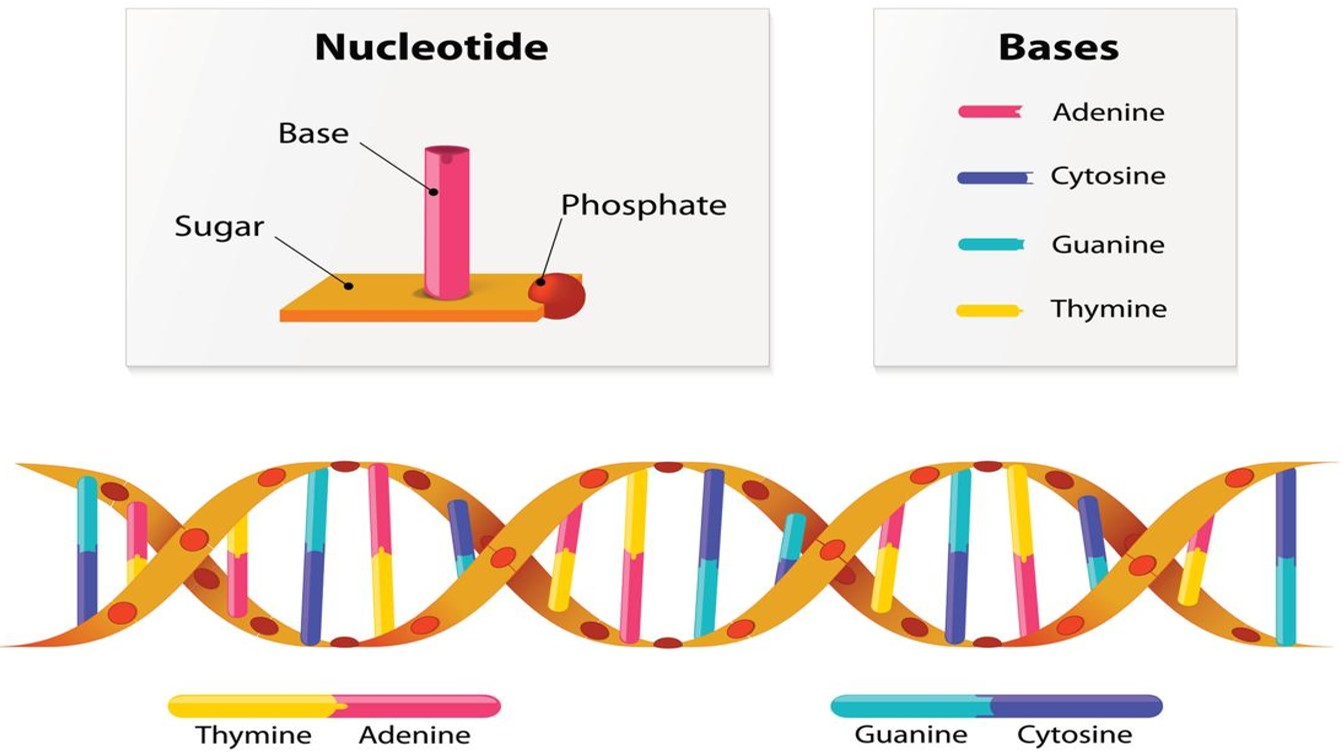
\includegraphics[width=\linewidth]{DNAStructure.jpg}
 	\caption{La struttura del DNA e del nucleotide.}
  	\label{fig:DnaAndNucleotideStructure}
\end{figure}
\newline
La struttura è caratterizzata da una doppia elica di lunghezza variabile, dove ciascun filamento è formato da una sequenza di molecole chiamate \textit{desossiribonucleotidi}.
\newline
Un desossiribonucleotide è composto da una molecola di zucchero, un gruppo fosfato ed una base azotata. Di quest'ultima, ne esistono quattro tipi:
\begin{itemize}
	\item \textit{adenina} (A);
	\item \textit{timina} (T);
	\item \textit{guanina} (G);
	\item \textit{citosina} (C).
\end{itemize}
Una proprietà importante delle basi azotate è che sono biunivocamente legate tra loro: l'Adenina si può legare solo con la Timina (A-T), mentre la Guanina con la Citosina (G-C). Questo significa che i filamenti sono complementari e quindi se conosciamo la sequenza di basi di un filamento di DNA sappiamo anche la sequenza di quello complementare.

\section{RNA}
L'\textit{RNA}, ovvero \textit{acido ribonucleico}, è una macromolecola caratterizzata da una struttura a singolo filamento composta da una sequenza di lunghezza variabile di \textit{ribonucleotidi}.
\newline
I ribonucleotidi si differenziano rispetto ai desossiribonucleotidi per una diversa molecola di zucchero e per la presenza della base azotata Uracile (U) che sostituisce la Timina.
\newline
Un tipo di RNA importante è l'\textit{RNA messaggero} (mRNA), che trasporta l'informazione genetica contenuta nel DNA in una regione cellulare (citoplasma) in cui avviene la sintesi delle proteine\footnote{La sintesi proteica è il processo attraverso il quale vengono prodotte nuove proteine.}.

\section{Proteine}
Le proteine sono le fondamenta di un organismo, infatti determinano la struttura e le funzioni delle cellule, ad esempio le cellule del cervello differiscono da quelle dei muscoli principalmente perché usano tipi diversi di proteine.
La loro struttura è composta da sequenze di \textit{aminoacidi} legati tra loro.
\newline
Sebbene esistano oltre cinquecento aminoacidi in natura, solo venti sono codificati dal codice genetico umano e pertanto utilizzati per la sintesi proteica.
\newline
La conversione dell'informazione genetica dal DNA in proteina, avviene in due processi, di seguito elencati:
\begin{enumerate}
	\item \textit{trascrizione}: viene prodotto l'RNA messaggero che trasporta l\?informazione nel citoplasma dove avverrà la traduzione;
	\item \textit{traduzione}: l'informazione contenuta all'interno del mRNA viene convertita in proteine.
\end{enumerate}